% This is samplepaper.tex, a sample chapter demonstrating the
% LLNCS macro package for Springer Computer Science proceedings;
% Version 2.21 of 2022/01/12
%
\documentclass[runningheads]{llncs}
%
\usepackage[T1]{fontenc}
% T1 fonts will be used to generate the final print and online PDFs,
% so please use T1 fonts in your manuscript whenever possible.
% Other font encondings may result in incorrect characters.
%
\usepackage{graphicx}
% Used for displaying a sample figure. If possible, figure files should
% be included in EPS format.
%
% If you use the hyperref package, please uncomment the following two lines
% to display URLs in blue roman font according to Springer's eBook style:
%\usepackage{color}
%\renewcommand\UrlFont{\color{blue}\rmfamily}
%\urlstyle{rm}
%
\begin{document}
%
\title{Reducing Intuitive-Physics Prediction Error through Playing}
%
\titlerunning{Reducing Prediction Error through Playing}
% If the paper title is too long for the running head, you can set
% an abbreviated paper title here
%
\author{Olivier L. Georgeon\inst{1, 2}\orcidID{0000-0003-4883-8702} \and
Paul Robertson\inst{3}\orcidID{0000-0002-4477-0379} }
%
\authorrunning{Georgeon and Robertson}
% First names are abbreviated in the running head.
% If there are more than two authors, 'et al.' is used.
%
\institute{UR CONFLUENCE: Sciences et Humanites (EA 1598), UCLy, France 
	\email{ogeorgeon@univ-catholyon.fr} \and
SyCoSMA, LIRIS, CNRS, Villeurbanne, France \and
DOLL Labs, Lexington, MA, USA\\
\email{paulr@dollabs.com}}
%
\maketitle              % typeset the header of the contribution
%
\begin{abstract}
We present an autonomous robot that generates behaviors to calibrate its intuitive-physics engine also known as the ``Game Engine in the Head'' (GEITH).
%The robot selects behaviors that yield information to refine the GEITH parameters. 
At the beginning of each interaction cycle, the robot uses its GEITH to run a simulation to compute predicted sensory signals. 
For each sensor, prediction error is the difference of the predicted sensory signal minus the actual sensory signal received at the end of the interaction cycle. 
Results show that over a few tens of interaction cycles, the robot improves its GEITH calibration and decreases its prediction errors. 
Moreover, the robot generates behaviors that human observers describe as playful.

\keywords{Active infernce  \and constructivist learning \and enaction \and intrinsic motivation \and robotics \and core knowledge.}
\end{abstract}
%
%
%
\section{Introduction}
\label{sec:intro}

It is widely believed that cognitive beings possess some kind of a \textit{world model} that they use to generate intelligent behaviors.
How they construct, maintain, and use this world model remains, however,  an open question in cognitive science and artificial intelligence. 

The Partially Observable Markov Decision Process (POMDP) literature has proposed a broad range of methods to infer a \textit{belief state} in a partially observable process.
%The belief state amounts to the agent's world model of the environment that the agent can only partially observe.  
The agent uses the belief state as a model of the environment that the agent observes through partial observations.  
If the agent knows the POMDP's state-transition function and the observation function \textit{a priori}, the problem of computing the belief state has been mathematically solved, but proved to be generally intractable (NP-Hard) \cite{astrom1965optimal}. 
% It was, however, also proven that the implementation of the solution becomes intractable as the set of states and observation grows. 
%Without knowledge of the state transition and observation functions, the problem of inferring belief states in POMDPs does not lend itself to a mathematical analysis. 

Karl Friston and his research group have proposed Active Inference \cite[e.g.]{smith_step-by-step_2022} as a method to interactively refine the world model by minimizing \textit{free energy}, or equivalently, prediction error and surprise \cite{friston_free-energy_2010}.
The world model %at step $t$ 
is represented as the distribution of probability %$\mu_t$ that gives the probability 
of each possible state of the world. 
In essence, at each instant, the agent estimates which states are the most or least likely to be the actual state of the world.
%$s \in S$ of all the possible states of the world. 
%This method iteratively updates $\mu_t$ on each interaction cycle.
%The agent selects the action that is expected to maximize the information gained to refine the probability distribution. 
%The estimation of expected information gained is computed through the variational free energy which involves a divergence between two probability distributions: the agent's world model $\mu$ and the joint probability distribution $g = P(O, S)$ of observations $O$ and world states $S$ called the \textit{generative model}. 
Active inference has been used in robotics \cite{lanillos_active_2021} but generally under \textit{closed-world} settings in the sense that the set of possible states is known \textit{a priori}---a requirement for most the active inference mathematical apparatus. 
%Significant challenges remain when the robot is placed in an open world. 
%and the relation from states to observations be known \textit{a priori}.
%---an assumption that we avoid in the present study. %$S$ 
%Moreover, computing the free energy remains too computationally intensive for our robotics experiment.
%remain; however to  and the high number of interaction cycles to converge to a useful world model makes this method inapplicable in our case of a robot interacting with the open world. 

When the robot is thrown in an open world, 
the POMDP and active inference literature suggest that it needs prior assumptions about the world to cope with complexity \cite{georgeon_artificial_2024}. 
The present study examines how the ``Game Engine In The head'' (GEITH) can work as a suitable prior assumption that an autonomous robot could use to maintain an open world model and reduce prediction errors. 

Joshua Tenenbaum and his research group have proposed the GEITH \cite{battaglia_simulation_2013} as the capacity of cognitive beings to simulate basic dynamics of physics and interactions. 
In the brain, the GEITH rests upon structures that are partially predefined by genes and then completed through ontogenetic development.  
Similarly, it is possible to endow artificial agents and robots with a predefined software game engine, and expect them to refine the parameters of their game engine as they test their predictions in the world.

This paper proposes an approach to designing autonomous agent that can refine their GEITH through their lifetime.
The refinement of the game engine is measured through two methods. 
The first is performed by the robot itself by measuring the prediction error of sensory signals. 
Decrease in prediction errors shows improvement of the game engine. 
The second is performed by the experimenter by assessing whether the game engine parameters converge towards a target range that indicates that the robot managed to calibrate its GEITH. 




\section{Our hypothesis}

We comply with active inference theory in several regards. 
Firstly, we do not consider sensory signals to be \textit{representational} of the world's state. 
%Different sensory signals may come out of the same environment state depending on the agent's action. 
% Each state of the world can generate different sensory signals depending on the action performed by the agent.
The world is hidden to the agent so that a given state can return contrary sensory signals when acted upon differently by the agent.
This implies a ``conceptual inversion'' of the interaction cycle in which action comes first and sensory signal comes second as an  \textit{outcome} of action. 
Secondly, we do not provide the agent with presupposed ontological knowledge about entities in the world. 
The agent must infer the existence and properties of entities by itself through patterns of interactive experience. 
This view can be traced back to Whitehead's process philosophy in which phenomenal experience involves abstracting entities out of events \cite{whitehead1929}. 
Thirdly, no extrinsic goal is encoded in the agent in the form of goal states that the agent should search based on reward or other criteria. 
We nonetheless may associate some \textit{prior preference} with interactions. 
In short, the agent has no \textit{rewarding world states} but has \textit{rewarding interactions}. % (positive or negative).
For a deeper examination of these principles in relation with the active inference literature, we refer the reader to our previous article \cite{georgeon_artificial_2024}.

We also adopt \textit{prediction error} as a measure of the quality of the agent's world model. %, and minimizing surprise is a powerful motivator. 
%Indeed, to survive, cognitive beings should avoid bad predictions as much as they can. %generally stay away from bad surprises.
As introduced in Section \ref{sec:intro}, however, we are not using gradient descent of prediction error (or surprise) as a motivational principle to drive the learning process. 
As we will develop, our agent is not always driven by a value optimization process; it may sometimes enact disinterested behaviors.
% We are investigating an alternative approach based on an innate set of behaviors that the robot may select depending on its \textit{emotional state}.  
For us, prediction-error reduction is not a means to improve the world model but a consequence of its improvement.

We are using a cognitive architecture that we designed previously based on sensorimotor and enactive principles \cite{georgeon_artificial_2024}. 
The present article reports the integration of the new GEITH module within this cognitive architecture as illustrated in Figure \ref{fig:geith}. 
The GEITH supports the simulation of behaviors before their selection by the cognitive architecture and their enaction by the robot. 
At the beginning of each interaction cycle, the simulation computes the \textit{predicted outcome}.
At the end of the interaction cycle, the predicted outcome is compared with the \textit{actual outcome} to compute the prediction error.   
We investigate the core elements of the GEITH that are needed for the agent to reduce prediction error. 

We draw inspiration from studies on \textit{core knowledge} in the brain of animals and human infants. 
For example, Elizabeth Spelke and her colleagues argued for the existence of two core systems of geometry that ``evolved before the emergence of the human species'':  
``The \textit{core navigation system} captures absolute distance and sense [..] but not relative length or angle; the \textit{core form analysis system} does the reverse'' \cite[p. 2789]{spelke_core_2012}.
We start by implementing the minimal requirements she deems necessary for both systems, namely the ability to handle points and lines in spatial memory, the foundational elements of Euclidean geometry. 

Our cognitive architecture encodes behaviors as \textit{composite interactions} which are sequences of \textit{primitive interactions}.
A primitive interaction is a \textit{control loop} that involves actuator commands, expected sensory feedback, spatio-temporal attributes, termination conditions, termination outcome, and prior preference. 
Examples are in Section \ref{sec:expe}. 
The GEITH may consider some outcomes as resulting from the interaction with ``something'' in the environment.
In this case, the GEITH instantiates a data structure called a \textit{phenomenon}\footnote{Common-sense usage of the term \textit{phenomenon}: ``something'' that a cognitive being perceives in the environment. Technically: ``any useful grouping of a subset of spatio-temporal patterns experienced by an agent in an environment'' \cite[p. 8]{thorisson_explanation_2021}.} and localizes this phenomenon at the position of the interaction in spatial memory.
Next, the GEITH simulates subsequent interactions with phenomena to predict future outcomes. 
The present study focuses on the simplest possible kind of phenomenon: points on the two-dimensional floor.

We seeded the cognitive architecture with ``innate'' composite interactions (Fig. \ref{fig:geith}, top-center) that cause the robot to explore the environment and to interact with points encountered on the floor. 
Here we do not examine the learning of new composite interactions (we did in other studies \cite{georgeon_cash_2019}) but only the refinement of the GEITH parameters to reduce prediction error.
The cognitive architecture uses variables that represent the robot's \textit{emotional state} to selects composite interactions to try to enact.

\begin{figure}
	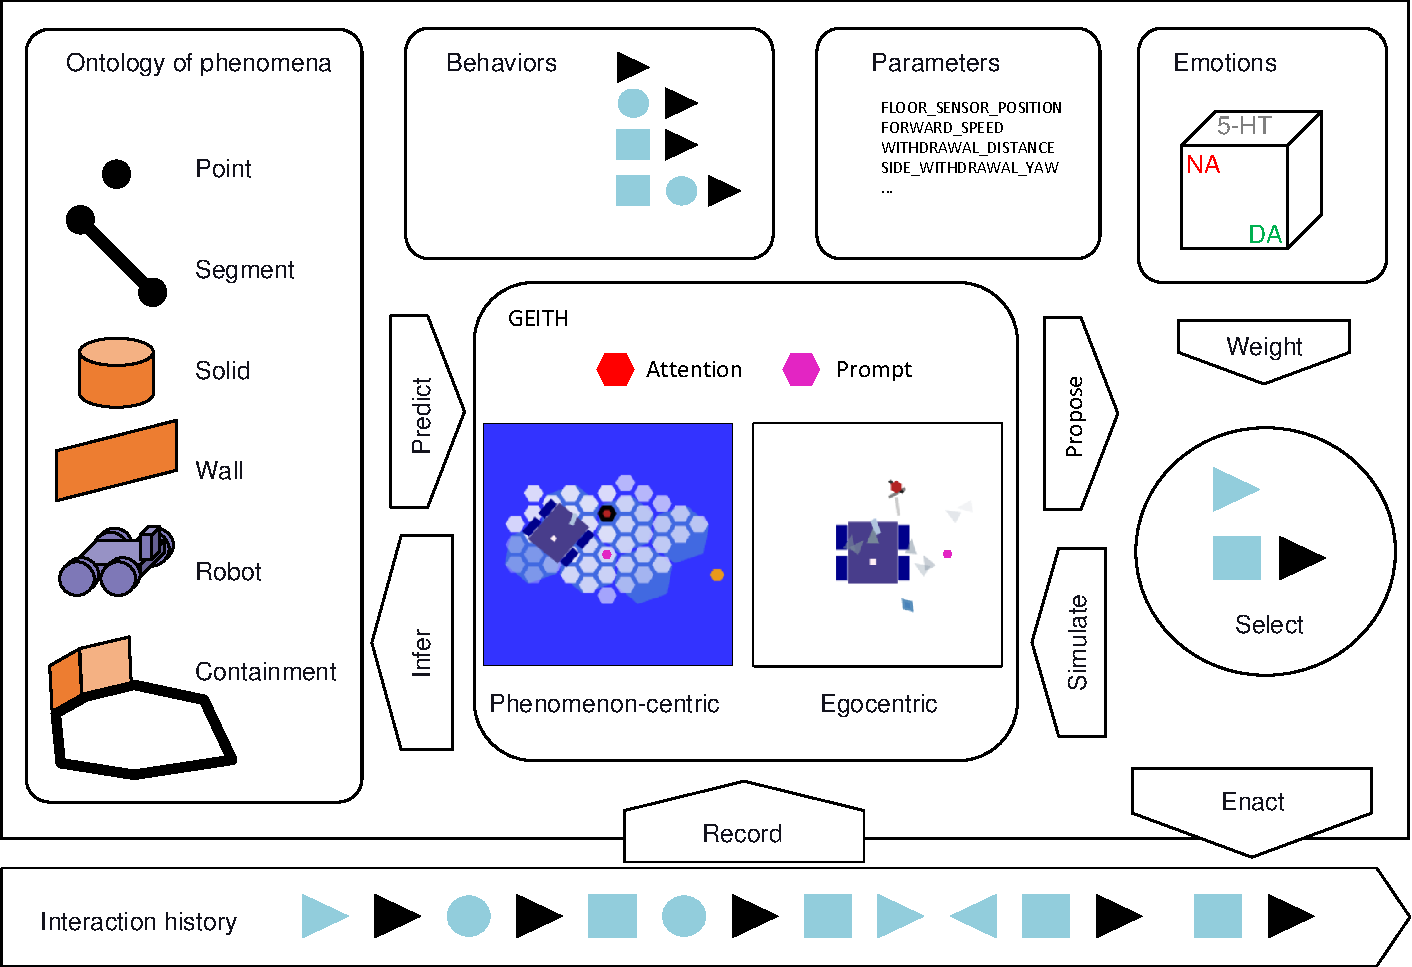
\includegraphics[width=\textwidth]{Figure_geith.pdf}
	\caption{The game engine within the cognitive architecture.
		Bottom: the history of interactions enacted over time.
		Rightward triangles: \texttt{forward}. Leftward triangles: \texttt{backward}. Squares: \texttt{swipe}. Circles: \texttt{turn}. Light-blue: \texttt{no\_tape}. Black: \texttt{tape}.
		Center: the GEITH.
		Red hexagon: the focus of attention localized at the position of the phenomenon. 
		Magenta hexagon: the prompt is the localization of the next selected interaction's destination: \texttt{swipe} to the right.
		Left: the types of phenomena inferred trough interactive experience.
		Solid objects, walls, and other robots can be detected by the echo-localization sensor but are not present in this experiment.
		Top center: predefined composite interactions and GEITH parameters.
		Top right: three-dimensional emotional state based on dopamine (DA), serotonin (5-HT), and nor-adrenaline (NA).
		Right: the decider selects the next behavior based on the emotional state and the expected outcome predicted by the GEITH.} \label{fig:geith}
\end{figure}

We use Hugo Lövheim's ``cube of emotions'' \cite{lovheim_new_2012} as a basic emotional model based on three neurotransmitters: dopamine (DA), serotonin (5-HT), and nor-adrenaline (NA) (Fig. \ref{fig:geith}, top right).
This model associates dopamine with pleasure and reward-seeking behavior, serotonin with well-being and playful behavior, and nor-adrenaline with arousal and stress responses.
It has been successfully used for simple emotional robotics.
Our robot visually indicates its predominant neurotransmitter level using an intuitive color code developed by Max Talanov and his team: green for dopamine, white for serotonin, red for noradrenaline, and blue when all three neurotransmitter levels are low \cite{chebotareva_emotional_2019}.

The GEITH implements two levels of spatial working memory: \textit{egocentric} and \textit{allo-phenomenon-centric} (Fig. \ref{fig:geith}, center).  
The interactions and displacements are received in the egocentric reference frame based on the position of sensors and translation speed given as GEITH parameters, and the yaw measured by the Inertial Measurement Unit (IMU) which plays a similar role as the vestibular system %. 
%Using spatial-displacement information, the GEITH updates the position of the recent history of interactions in egocentric memory 
(Fig. \ref{fig:video}, top right).
When the robot encounters a new phenomenon, the GEITH instantiates a new allocentric reference frame centered on this phenomenon to track the displacement of the robot relative to this phenomenon (Fig. \ref{fig:video}, bottom right). 
This mechanism of coordinate conversion relates to that implemented by Howard Schneider's in his Causal Cognitive Architecture \cite{schneider_emergence_2024}, and to 
Jeff Hawkins' thousand brain hypothesis \cite{hawkins_framework_2019} according to which the brain records thousands of small spatial models to memorize interactions with different kinds of objects.
%We implemented Tenenbaum's idea to give a \textit{sleep}/\textit{awake} attribute to phenomena. If the GEITH detects that the phenomenon moves, it switches the attribute to \textit{awake}.

Once the robot has selected an object in the environment, its serotonin level increases which triggers behaviors of interactions with this object to calibrate its GEITH parameters. 
Phenomenon-centric memory is discretized into an hexagonal grid inspired by grid cells in the brain. 
The cognitive architecture uses this grid as a small finite discrete POMDP in which to perform information seeking and optimization with an algorithm off the shelf. 



\section{Experiment}
\label{sec:expe}

We designed a robotic platform called Petitcat\footnote{Sections \ref{sec:expe} and \ref{sec:results} personalize the robot by name and pronoun to enhance readability. We do not claim that he has a psychology or gender.} based on the ``robot car'' commercialized by Osoyoo \cite{osoyoo_robot_car}.
The experiment reported here uses only two sensors.
The ``floor luminosity sensor'' is a bar of 5 infrared-reflective sensors directed to the floor.
From this bar of sensors we retrieve 4 possible states:  \texttt{none},  \texttt{left},  \texttt{front}, or \texttt{right} indicating the possible presence and relative position of a black tape beneath them.  
The IMU measures the yaw during the enaction of interactions.
Note that Petitcat cannot see the tape from a distance. 
He has no camera, lidar or odometer.
What looks like eyes on his head is an ultrasonic echo-localization sensor not used in this experiment. 
We added an RGB LED as the emotion indicator (Fig. \ref{fig:video}). 

\begin{figure}
	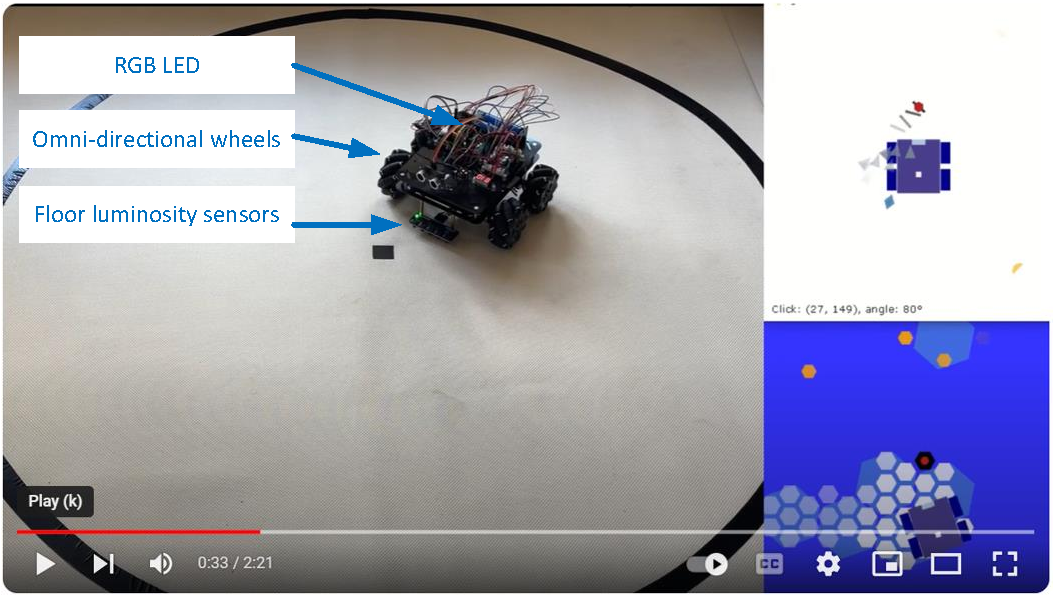
\includegraphics[width=\textwidth]{Figure_video.pdf}
	\caption{Screenshot of a video example run \cite{georgeon_petitcat_2024}.
		Left: Petitcat playing with a point made of a piece of black tape on the floor.
		Top right: Petitcat's egocentric memory. Black segments: black tape detection events. 
		Bottom right: phenomenon-centric memory. 
		Black hexagon: the point phenomenon used as origin of the allocentric reference frame. 
		Yellow hexagons: echo measured with the sonar. Red hexagon: focus of attention.} \label{fig:video}
\end{figure}

The C++ software running on the robot's Arduino board controls the enaction of primitive interactions. 
A personal computer implements the GEITH and the cognitive architecture that remote controls the robot through wifi.
The cognitive architecture selects the primitive interaction to try to enact and sends it to the robot. 
The robot tries to enact it and sends the outcome back to the PC.  
The code is open source and shared online \cite{petitcat_github}.

For this experiment, we defined four possible commands: \texttt{forward}, \texttt{backward}, \texttt{swipe}, and \texttt{turn}. 
\texttt{Forward} and \texttt{backward} are longitudinal translations. Their spatio-temporal attribute is the target duration (float).   
\texttt{Swipe} is a lateral translation. Its spatio-temporal attributes are the direction (left or right) and target duration (float). 
\texttt{Turn} consists in turning in place. Its spatio-temporal attribute is the target yaw (float), negative when counter-trigonometric. 
%they have been separated rather than using a direction attribute because they are conceptually different: moving toward or away from a target. 

The control loop monitors the elapsed time, the yaw, and the floor luminosity. %, and the distance of echo signals during the enaction of interactions. 
The termination conditions are reaching the target duration or yaw, or detecting the black tape, making two possible outcomes: \texttt{no\_tape} or \texttt{tape}.
This gives eight primitive interactions identified by their tuple $\langle$command, outcome$\rangle$ (4 commands $\times$ 2 outcomes).
% Note that Petitcat cannot ``see'' the tape but only ``feel'' it through its floor luminosity sensors when he passes over it.
All interactions are given a zero prior preference except $\langle$\texttt{forward}, \texttt{no\_tape}$\rangle$ which has a positive one.
Additionally, the robot returns the measured spatio-temporal attributes: measured duration (float), measured yaw (float), and black tape detection (none, left, front, right). 

When the black tape is detected, the movement is interrupted and a ``reflex'' movement is performed to withdraw away from the tape by a few centimeters. 
When the detection is on the side, this withdrawal includes a rotation to the opposite side, which tends to bring the robot back into a position perpendicular to the tape. This behavior was implemented to prevent the robot from falling off a table or exiting the arena.

We seeded the cognitive architecture with the four composite interactions below, which constitute ``innate'' manners for Petitcat to interact with points. 
The GEITH tries to simulate them, computes their spatio-temporal attributes according to the position of the phenomenon in memory, and proposes those that are feasible in the current context.
\begin{enumerate}
	\item $\langle\langle$\texttt{forward}, \texttt{tape}$\rangle\rangle$
	\item $\langle\langle$\texttt{turn}, \texttt{no\_tape}$\rangle$, $\langle$\texttt{forward}, \texttt{tape}$\rangle\rangle$
	\item $\langle\langle$\texttt{swipe}, \texttt{no\_tape}$\rangle$, $\langle$\texttt{forward}, \texttt{tape}$\rangle\rangle$
	\item $\langle\langle$\texttt{swipe}, \texttt{no\_tape}$\rangle$, $\langle$\texttt{turn}, \texttt{no\_tape}$\rangle$, $\langle$\texttt{forward}, \texttt{tape}$\rangle\rangle$. 
\end{enumerate}

The levels of the neurotransmitters can vary from 0 to 100 and are initialized at 50. DA prevails in case of equality.
Prevalence of DA makes Petitcat initially select the $\langle$\texttt{forward}, \texttt{no\_tape}$\rangle$ interaction because it has a positive prior preference.
When he detects a point (by surprise), 5-HT increases to its max. 
Prevalence of 5-HT and the presence of a point phenomenon in memory triggers the selection of the innate interactions with the point.
If the prediction errors do not decrease (i.e., prediction does not improve), 5-HT decreases.
When 5-HT drops below or equal to DA, the  $\langle$\texttt{forward}, \texttt{no\_tape}$\rangle$ interaction is again selected causing Petitcat to go explore new destinations. 

Prediction errors may concern both the outcome of primitive interactions and the spatio-temporal measures.
Prediction errors on the outcome (\texttt{tape} predicted but \texttt{no\_tape} occurred, or the reverse) mean that the selected primitive interaction failed and another interaction was actually enacted instead. 
Failing primitive interactions cause the composite interaction to which they belong to abort, and the NA level to increase to its max.

The GEITH uses a \textit{focus of attention} point and a \textit{prompt} point to compute the spatio-temporal attributes of interactions (Fig. \ref{fig:geith}, center). 
When Petitcat interacts with a point, the GEITH places the focus of attention at the place of the phenomenon. 
A failure to interact with the point means that the localization of the phenomenon in memory is erroneous. 
%generally due to drift caused by inaccuracy in the GEITH parameters and the spatio-temporal measures. 
The high NA level that occurs in case of failure causes the GEITH to move the focus of attention to another cell in phenomenon-centric memory in search for the point.
Cells compete to catch the focus with preference given to those closer to the last detected position of the phenomenon but having gone the longest period since last being visited.
The interactions with the point continue afterward based on focus in different cells. 
NA is reset to 50 if Petitcat finds the lost point, otherwise it progressively decreases until it drops below 50 causing Petitcat to abandon the search. 

In addition to the number of failed interactions, we also expect the prediction errors of the yaw and of the forward duration to decrease as the GEITH adjusts its parameters. 
Our GEITH has about 20 parameters but this experiment only involves \texttt{FLOOR\_SENSOR\_POSITION}, \texttt{FORWARD\_SPEED}, \texttt{WITHDRAWAL\_DIS\-TANCE}, and \texttt{SIDE\_WITH\-DRA\-WAL\_YAW}.
Note that the GEITH has no means to infer the absolute values of these parameters but can only adjust them in relation to one another.
The GEITH cannot either predict that the point will be detected on the side of the floor luminosity sensor which will cause a withdrawal with rotation. The GEITH can only make the robot aim strait at the point and thus always predicts straight withdrawal. 

%Ideally, we would like the GEITH to find by itself the relations of causality that link parameters to prediction errors, but in this experiment, we predefined these relations.


\section{Results}
\label{sec:results}

Several videos of experiment runs are available online. 
Here we analyze the representative run recorded in \cite{georgeon_petitcat_2024}.
In this run, Petitcat encountered the point on Step 2 and interacted with it up to Step 60.
On Step 17, it missed the point but found it again on Step 20.
This is shown in the \textit{outcome code prediction error plot} in Fig. \ref{fig:outcome}. 
The fact that Peticat did not miss the point after Step 20 shows an improvement of the GEITH parameters.

\begin{figure}
	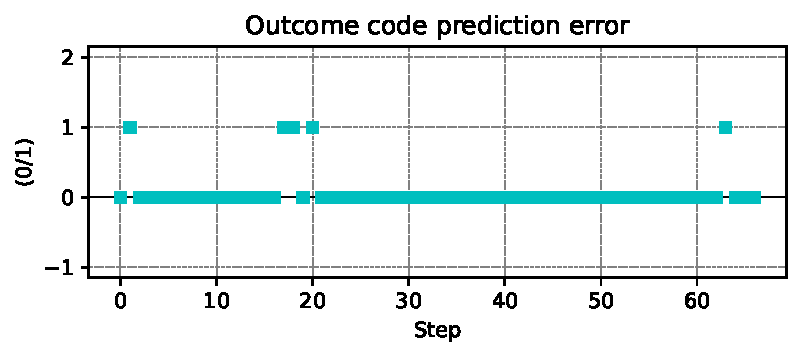
\includegraphics[width=\textwidth]{01_Outcome_code.pdf}
	\caption{Outcome prediction error plot: 0 if predicted outcome = actual outcome (successful interaction), 1 otherwise (failed interaction).
	Step 2: Petitcat did not expect to detect the point.
	Steps 17: he expected to detect the point while translating forward but missed it.
	Steps 18: he expected to not detect the point while turning but detected it.
	Step 20: he did not predict detecting the point but did. 
	Step 63: As he moved away from the point, he did not expect to detect the arena border. } \label{fig:outcome}
\end{figure}

As explained above, the GEITH cannot predict when Peticat will detect the point on the side. 
This can cause large yaw prediction errors because the robot unexpectedly turned during withdrawal.
Fig. \ref{fig:yaw_pe} shows these prediction errors that do not improve over time. 

\begin{figure}
	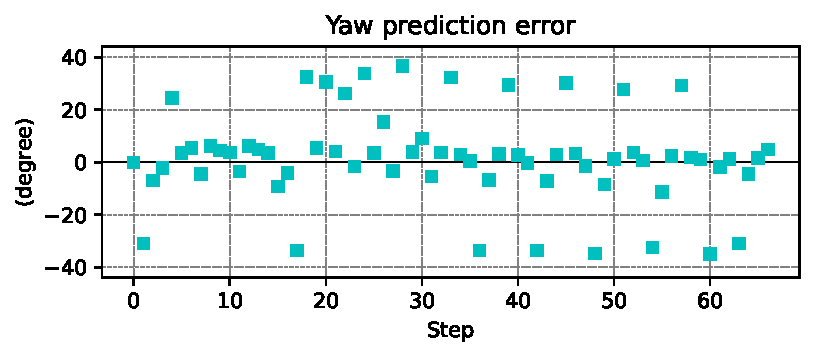
\includegraphics[width=\textwidth]{02_yaw_pe.pdf}
	\caption{Yaw prediction error plot. The prediction errors come from different causes which makes the interpretation of the plot difficult. 
		Points above 20 or below -20 are large prediction errors occurring when Petitcat turned while withdrawing because the GEITH does not prediction detecting the point on the side.
	%	Step 2: Petitcat detected the point on the side which caused an unpredicted yaw to the left.   shows no improvement when we do not distinguish between the different kinds of interactions.
	} \label{fig:yaw_pe}
\end{figure}

The GEITH simulates turning while withdrawing based on the \texttt{SIDE\_WITH\-DRA\-WAL\_YAW} parameters.
To adjust this parameter, the GEITH must 
%isolate the interactions in which he detected the point on the side and 
compute the \textit{yaw residual error} 
%The yaw residual error is the residual prediction error 
that is left when knowing on which side the point was detected. 
Fig. \ref{fig:yaw_re} shows that the yaw residual error decreases as the robot adjusts the \texttt{SIDE\_WITH\-DRA\-WAL\_YAW} parameter.

\begin{figure}
	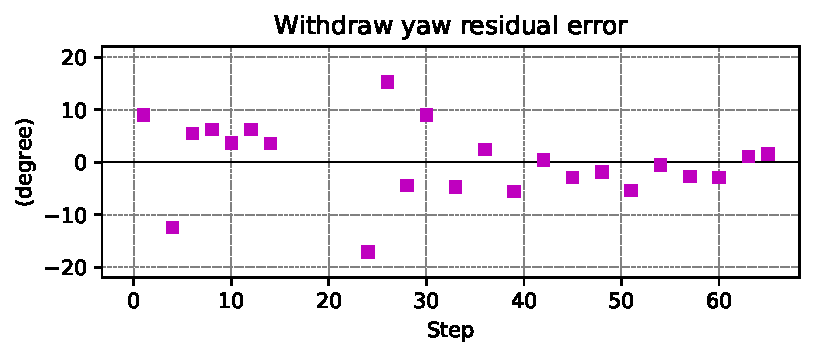
\includegraphics[width=\textwidth]{03_yaw_re.pdf}
	\caption{Yaw residual error of interactions that have a \texttt{tape} outcome. 
		It shows a significant decrease as the robot interacts with the point.
	} \label{fig:yaw_re}
\end{figure}

The adjustment of \texttt{FORWARD\_SPEED} and \texttt{WITHDRAWAL\_DIS\-TANCE} allows for a visible decrease of the forward duration prediction error shown in Fig. \ref{fig:forward_re}.

\begin{figure}
	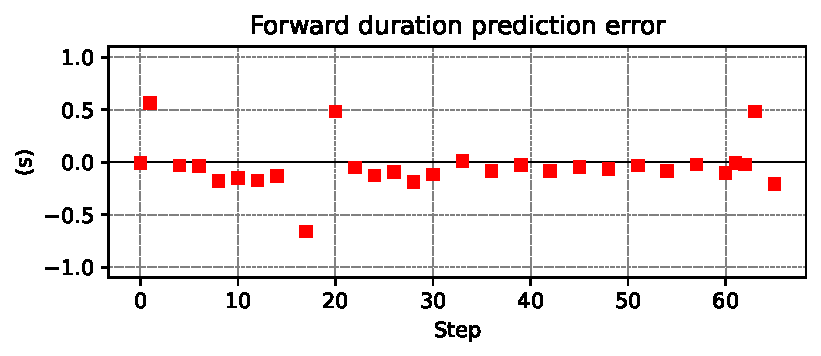
\includegraphics[width=\textwidth]{07_Forward_duration_pe.pdf}
	\caption{Duration prediction error for \texttt{forward} interactions.
	Step 2 and 20: the forward translation was unexpectedly interrupted by the point detection.
	Step 17: the forward duration was longer than expected because the robot did not detect the point.
	Except for these events, the plot shows that the forward duration prediction error decreases.
	From Step 63: Forward duration prediction errors occur as Petitcat discovers the arena border.
	} \label{fig:forward_re}
\end{figure}

%\begin{figure}
%	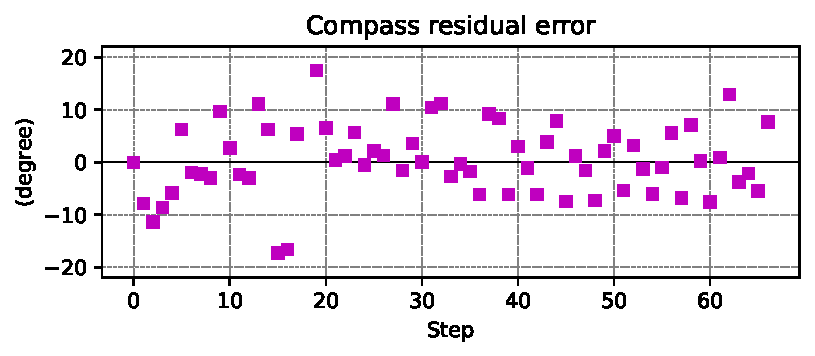
\includegraphics[width=\textwidth]{04_Compass.pdf}
%	\caption{The compass residual error decreases after step 20 when the robot starts circling around the point.
%	It nonetheless remains noisy due to sensor imprecision.
%	The sliding average over 10 interactions tends to 0.8° and the standard deviation to 7.4°.} \label{fig:compass}
%\end{figure}

\section{Conclusion}

We demonstrated a simple robot that managed to reduce intuitive-physics prediction errors in an open environment. 
We drew inspiration from theories positing core knowledge in the brain that have innate origins.
The robot's design rests upon the cognitive architecture, the game engine, the model of emotions, and an innate set of behaviors.
These elements are hard-coded in the robot but what is not predefined is the set of world states and the ontology of objects in the world.

When the robot finds an object, it instantiates a small local model in the reference frame of this object. 
This finite discrete model lends itself to regular active inference techniques. 
We continue studying how to optimize the process of GEITH refinement in such local models using the active inference python library  \texttt{inferac\-tively-pymdp} \cite{Heins2022}.


This study merely begins to explore the intricacies involved in autonomously refining the world model.
We expect the next step to involve endowing the robot with the capacity to represent lines between points which could open the way to learning compositionality of phenomena. 
Next we shall examine how the robot can deal with persistence, disappearance, or displacement of objects. 

We are not claiming the robot can actually \textit{experience} emotions let alone have sentience. 
Our approach, nonetheless, helps generate behaviors that human observers easily interpret as lifelike, which could find applications in companion robotics.
The robot seems to enjoy exploring for the mere pleasure of movement as it lights up in green (DA prevails); 
it plays with the point as for developing its skills as it lights up in white (5-HT prevails); 
it seems anxious to find the lost point as it lights up in red (NA prevails). 
We wish to further study to what extent observers attribute these subjective traits in future experiments.
%It wish to further investigate how human observers project these interpretations in a controlled experiment. 



%Prediction errors may have a variety of causes sometimes difficult to untangle. 
%Again, we are looking for core systems of causal explanation that may have evolved in the brain.
%The literature has pointed out that explanation requires isolating relevant elements of context, and tracking their transformation through series of events \cite{thorisson_explanation_2021}. 
%Explanation may also involve a confrontation between proponent and opponent arguments, and further interactions with the world to weigh these arguments. 




\begin{credits}

%\subsubsection{\ackname} A bold run-in heading in small font size at the end of the paper is
%used for general acknowledgments, for example: This study was funded
%by X (grant number Y).

%\subsubsection{\discintname}
%It is now necessary to declare any competing interests or to specifically
%state that the authors have no competing interests. Please place the
%statement with a bold run-in heading in small font size beneath the
%(optional) acknowledgments\footnote{If EquinOCS, our proceedings submission
%system, is used, then the disclaimer can be provided directly in the system.},
%for example: The authors have no competing interests to declare that are
%relevant to the content of this article. Or: Author A has received research
%grants from Company W. Author B has received a speaker honorarium from
%Company X and owns stock in Company Y. Author C is a member of committee Z.
\end{credits}
%
% ---- Bibliography ----
%
% BibTeX users should specify bibliography style 'splncs04'.
% References will then be sorted and formatted in the correct style.
%
\bibliographystyle{splncs04}
\bibliography{georgeon.bib}
%
\end{document}
